\section{Experiments}
\label{sec:experiments}

\begin{figure*}[!t]
  \centering
  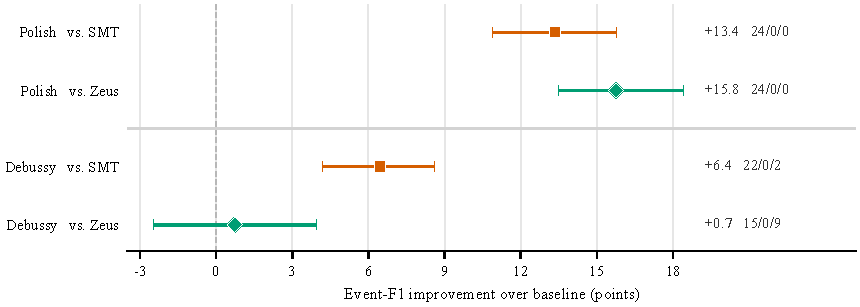
\includegraphics[width=0.86\textwidth]{figure/zero_shot_main_results.pdf}
  \caption{Paired Event-F1 improvements over each baseline. Bars are 95\% bootstrap intervals; annotations give the mean difference and wins/ties/losses.}
  \label{fig:zero-shot-summary}
\end{figure*}

\subsection{Protocol and Baselines}
We study transfer from a source domain $\mathcal{D}_s$ to held-out target test sets $\mathcal{D}_t$. No target test image is used for training or checkpoint selection; dataset adapters and run-time settings are fixed before test evaluation and disclosed below. Because the methods emit heterogeneous sequences, every valid output is projected to a multiset of pitch--duration events. For multiset intersection $M$ and predicted/reference counts $P,G$, we report
\begin{equation}
 \mathrm{EventF1}=100\frac{2M}{P+G}.
\end{equation}
This order-invariant measure isolates content recovery; SER and normalized tree-edit distance (TEDn) additionally assess ordering and hierarchy on OLiMPiC. All methods receive identical images and deterministic preprocessing, failed outputs remain in the denominator, and reported baseline values come from local inference. Differences use 10,000 paired bootstrap resamples over systems/pages and are significant only when the 95\% interval excludes zero.

Table~\ref{tab:datasets} summarizes the target domains and evaluation roles. We compare RIGOR-OMR with the released FP-GrandStaff checkpoint of SMT~\cite{riosvila2024smt} and the GrandStaff-LMX checkpoint of Zeus~\cite{mayer2024practical}.

\begin{center}
\begin{minipage}{\columnwidth}
\captionof{table}{Evaluation domains, sizes, and experimental roles.}
\label{tab:datasets}
\centering
\small
\setlength{\tabcolsep}{3pt}
\begin{tabular}{@{}llrl@{}}
\toprule
Dataset & Target domain & $N$ & Role \\
\midrule
Polish & historical scans & 24 & comparison \\
Debussy & unseen editions & 24 & comparison/ablation \\
GrandStaff & clean rendered & 200 & relation transfer \\
OLiMPiC & mixed systems & 200 & strict/relations \\
\bottomrule
\end{tabular}
\end{minipage}
\end{center}


\subsection{Comparison}
\begin{center}
\begin{minipage}{\columnwidth}
\captionof{table}{Zero-shot pitch--duration content recovery on Polish and Debussy.}
\label{tab:zero-shot}
\centering
\small
\setlength{\tabcolsep}{2.5pt}
\begin{tabular}{@{}llrrrr@{}}
\toprule
Target & Method & Prec. & Rec. & F1 & Pred./Gold \\
\midrule
Polish & RIGOR-OMR & \textbf{18.734} & \textbf{15.700} & \textbf{17.083} & 0.838 \\
 & SMT & 2.733 & 5.879 & 3.731 & 2.151 \\
 & Zeus & 3.971 & 0.800 & 1.332 & 0.202 \\
\midrule
Debussy & RIGOR-OMR & 7.058 & \textbf{10.737} & \textbf{8.517} & 1.521 \\
 & SMT & 1.277 & 5.432 & 2.068 & 4.252 \\
 & Zeus & \textbf{7.463} & 8.126 & 7.781 & 1.089 \\
\bottomrule
\end{tabular}
\end{minipage}
\end{center}


Table~\ref{tab:zero-shot} gives the central comparison. On Polish, RIGOR-OMR recovers 1,589 matching events and reaches 17.083 Event-F1, improving over SMT and Zeus by 13.352 and 15.751 points with intervals $[10.891,15.774]$ and $[13.477,18.422]$. On Debussy it reaches 8.517, exceeding SMT by 6.449 points ($[4.200,8.585]$) and remaining comparable to Zeus. The output ratios expose complementary failure modes: SMT over-generates on Debussy (4.252), whereas Zeus under-generates on Polish (0.202); RIGOR-OMR remains closer to the reference volume on both targets.

The aggregate intervals do not show how consistently the gain appears across individual pages or systems. Figure~\ref{fig:paired-f1} therefore retains the paired item-level differences. Polish separates cleanly from both baselines; on Debussy, RIGOR-OMR consistently exceeds SMT, whereas the comparison with Zeus contains both wins and losses and overlaps zero at corpus level.

\begin{figure*}[!t]
  \centering
  \begin{minipage}{\textwidth}
    \centering
    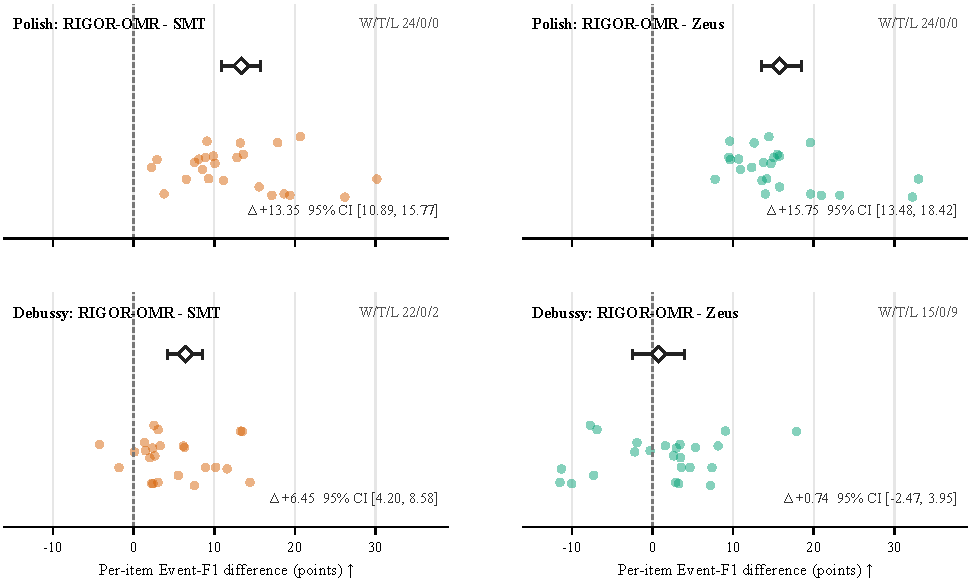
\includegraphics[width=0.98\textwidth]{figure/per_item_difference_small_multiples.pdf}
    \captionof{figure}{Per-item zero-shot Event-F1 differences. Positive values favor RIGOR-OMR; dots are held-out pages or systems, and diamonds/bars give the corpus difference and paired 95\% bootstrap interval.}
    \label{fig:paired-f1}
  \end{minipage}

  \vspace{0.7em}

  \begin{minipage}{\textwidth}
    \centering
    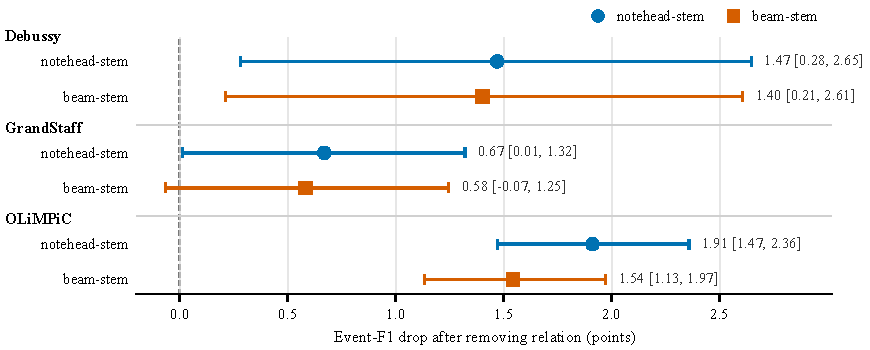
\includegraphics[width=0.86\textwidth]{figure/cross_domain_relation_forest.pdf}
    \captionof{figure}{Event-F1 decrease after removing a relation family from frozen full-pipeline outputs. Points are corpus differences and bars are paired 95\% intervals.}
    \label{fig:edge-forest}
  \end{minipage}
\end{figure*}

Order-invariant recovery does not establish globally correct notation. Table~\ref{tab:strict} therefore reports strict OLiMPiC evaluation. RIGOR-OMR completes all 200 conversions and outperforms SMT, but Zeus remains substantially stronger in SER, Event-F1, and TEDn. Thus the transferable local geometry produces evaluable structure without solving global ordering or hierarchy.

\begin{center}
\begin{minipage}{\columnwidth}
\captionof{table}{Strict OLiMPiC test200 results. Lower SER/TEDn and higher Event-F1 are better.}
\label{tab:strict}
\centering
\small
\setlength{\tabcolsep}{4pt}
\begin{tabular}{lrrrr}
\toprule
Method & SER & No tup. & Event-F1 & TEDn \\
\midrule
RIGOR-OMR & 74.421 & 73.574 & 8.786 & 61.342 \\
SMT & 100.000 & -- & 0.000 & 100.000 \\
Zeus & \textbf{56.486} & \textbf{50.625} & \textbf{48.242} & \textbf{47.751} \\
\bottomrule
\end{tabular}
\end{minipage}
\end{center}


\subsection{Ablation}
\label{sec:factorial}
The Debussy factorial evaluates staff geometry (A), detection (B), SAM2 refinement (C), and relation reasoning (D). A and B form a non-separable perception gate: A assigns instances to staff-normalized coordinates needed for pitch and grouping, while B supplies those instances. Without either, no valid pitch--duration event can be formed. The 12 configurations with $A=0$ or $B=0$ are therefore structurally equivalent zero-output cases and are losslessly collapsed into one row of Table~\ref{tab:factorial}; all four valid $AB\times C\times D$ combinations remain visible.

\begin{center}
\begin{minipage}{\columnwidth}
\captionof{table}{Debussy factorial ablation. A/B form the perception gate; C is SAM2 and D is relation reasoning.}
\label{tab:factorial}
\centering
\small
\setlength{\tabcolsep}{2.2pt}
\begin{tabular}{@{}lrrrr@{}}
\toprule
Variant & Prec. & Rec. & F1 & Pred./Gold \\
\midrule
$AB{+}C{+}D$ & 7.058 & \textbf{10.737} & 8.517 & 1.521 \\
$AB{+}D$ & \textbf{7.113} & 10.695 & \textbf{8.544} & 1.504 \\
$AB{+}C$ & 8.437 & 2.568 & 3.938 & 0.304 \\
$AB$ & 8.437 & 2.568 & 3.938 & 0.304 \\
$A{=}0$ or $B{=}0$ (12) & 0.000 & 0.000 & 0.000 & 0.000 \\
\bottomrule
\end{tabular}
\end{minipage}
\end{center}


With the full $AB{+}C{+}D$ path, Event-F1 is 8.517. Removing D lowers it to 3.938 ($-4.579$, paired interval $[2.288,7.019]$) as recall falls from 10.737 to 2.568, showing that isolated symbols do not recover complete events. Removing C instead changes 8.517 to 8.544 ($+0.027$, $[-0.614,0.793]$). SAM2 therefore supplies inspectable geometry, while the verified endpoint gain comes from relation reasoning.

We next remove one relation family from cached full-pipeline outputs and deterministically reconstruct without rerunning vision. Figure~\ref{fig:edge-forest} visualizes the effect and Table~\ref{tab:edges} retains the complete scores. Notehead--stem edges transfer most consistently; beam--stem edges improve Debussy and OLiMPiC and have a positive but interval-overlapping effect on GrandStaff. Slur/tie removal is neutral under the pitch--duration projection.
\label{sec:relations}

\begin{center}
\begin{minipage}{\columnwidth}
\captionof{table}{Complete relation ablation under frozen visual predictions. $\Delta$ is full minus ablated Event-F1; bold intervals exclude zero.}
\label{tab:edges}
\centering
\footnotesize
\setlength{\tabcolsep}{1.0pt}
\begin{tabular}{@{}llrrr@{}}
\toprule
Target & Removed & Full & $-$edge & $\Delta$ [95\% CI] \\
\midrule
Deb. & note--stem & 8.517 & 7.047 & \textbf{1.470 [0.282,2.647]} \\
Deb. & beam--stem & 8.517 & 7.114 & \textbf{1.403 [0.212,2.607]} \\
Deb. & slur/tie & 8.517 & 8.517 & 0.000 [0.000,0.000] \\
GS & note--stem & 8.887 & 8.217 & \textbf{0.669 [0.013,1.321]} \\
GS & beam--stem & 8.887 & 8.304 & 0.583 [$-0.067$,1.246] \\
OLi. & note--stem & 9.624 & 7.713 & \textbf{1.911 [1.472,2.358]} \\
OLi. & beam--stem & 9.624 & 8.082 & \textbf{1.543 [1.132,1.972]} \\
\bottomrule
\end{tabular}
\end{minipage}
\end{center}


\begin{center}
\begin{minipage}{\columnwidth}
\captionof{table}{Frozen relation inventory as edge count / affected pages.}
\label{tab:edge-inventory}
\centering
\footnotesize
\setlength{\tabcolsep}{1.5pt}
\begin{tabular}{@{}lrrrr@{}}
\toprule
Target & Note--stem & Beam--stem & Slur/tie & Ledger--note \\
\midrule
Deb.-24 & 3900/24 & 585/23 & 128/21 & inactive \\
GS-200 & 14947/200 & 2395/192 & 198/83 & 4/4 \\
OLi.-200 & 30113/200 & 333/111 & 266/117 & 8252/200 \\
\bottomrule
\end{tabular}
\end{minipage}
\end{center}


All edge ablations reuse frozen visual outputs and deterministically rebuild the prediction. Debussy intervals use 10,000 resamples with seed 20260720; both 200-item reproduction gates complete without failed pages. The ablation-specific OLiMPiC full score is not pooled with the official-style score in Table~\ref{tab:strict}.

\subsection{Implementation and Reproducibility}
Table~\ref{tab:implementation-settings} records the settings needed to distinguish the reported runs. They share the same OMR-trained DEIM--D-FINE checkpoint, 58-class taxonomy, staff geometry, and relation code, while page inference and maximum retained detections are logged per corpus rather than presented as identical. The detector operates at $640\!\times\!640$, uses score threshold $0.05$, and merges overlapping predictions with class-wise NMS at IoU $0.50$.

\begin{center}
\begin{minipage}{\columnwidth}
\captionof{table}{Frozen implementation settings for the reported modular runs.}
\label{tab:implementation-settings}
\centering
\footnotesize
\setlength{\tabcolsep}{2.6pt}
\begin{tabular}{@{}ll@{}}
\toprule
Component & Setting \\
\midrule
Detector & DEIM--D-FINE; 58 classes; $640\!\times\!640$ input \\
Filtering & score $0.05$; class-wise NMS IoU $0.50$ \\
Debussy & auto page mode; at most 1,000 detections \\
GrandStaff & $1280$-px tiles; $0.25$ overlap; at most 2,000 \\
Mask refiner & frozen SAM2.1 Hiera-Tiny; box-only prompt \\
Reconstruction & deterministic typed local rules \\
\bottomrule
\end{tabular}
\end{minipage}
\end{center}


Every fused box is processed by frozen SAM2.1 Hiera-Tiny with the box-only prompt used by the main runs. Masks provide area, orientation, skeleton, and endpoint measurements; a failed or empty refinement falls back to box geometry. Relation construction is local and deterministic: notehead--stem candidates use a distance threshold $\max(8\text{ px},1.35s)$, and beam--stem candidates use $\max(5\text{ px},0.45s)$ around an expanded beam support. A beam group is retained only with at least two stems. No Hungarian matching, integer program, message passing, or graph neural network is used.

\begin{figure*}[!t]
  \centering
  
\includegraphics[width=0.95\textwidth]{figure/debussy_qualitative_pipeline.pdf}
  \caption{Debussy \texttt{test\_0006}: (a) full-system overlay and selected crop; (b--f) staff geometry, accepted symbols, SAM2 masks, typed relations, and graph reconstruction. Masks are inspectable intermediates, not endpoint evidence.}
  \label{fig:qualitative-pipeline}
\end{figure*}

\subsection{Qualitative and Diagnostic Analysis}
Figure~\ref{fig:qualitative-pipeline} follows the best Debussy system (\texttt{test\_0006}, Event-F1 24.473). Its crop exposes staff localization, two noteheads, two geometry-derived stems, one beam, SAM2 masks, and the stored graph. Reconstruction composes notehead--stem and beam--stem edges, without a direct notehead--beam predictor.

Figure~\ref{fig:pitch-duration} separates recovery from binding. Pitch/duration F1 is 26.119/33.901 for RIGOR-OMR, 4.553/16.530 for SMT, and 20.318/29.550 for Zeus; count-correct scores are 11.118, 5.562, and 9.234. Yet joint F1 is 8.517: 527 events have correct pitch but unmatched duration, and 760 the converse, leaving exploitable binding headroom.

\begin{center}
\begin{minipage}{\columnwidth}
  \centering
  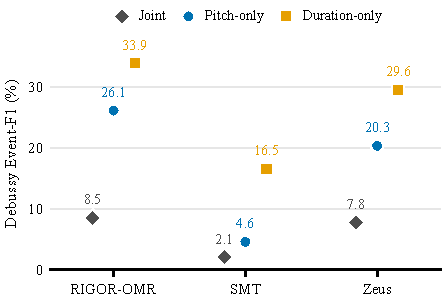
\includegraphics[width=0.90\columnwidth]{figure/debussy_binding_gap.pdf}
  \captionof{figure}{Joint, pitch-only, and duration-only Event-F1 on Debussy; marginal recovery reveals binding headroom.}
  \label{fig:pitch-duration}
\end{minipage}
\end{center}

\begin{center}
\begin{minipage}{\columnwidth}
\captionof{table}{Retained artifacts used to audit the modular prediction path.}
\label{tab:artifact-audit}
\centering
\footnotesize
\setlength{\tabcolsep}{2.3pt}
\begin{tabular}{@{}lll@{}}
\toprule
Stage & Retained evidence & Audited role \\
\midrule
Staff & lines, spacing, regions & normalization \\
Detection & class, box, confidence & symbol proposal \\
Mask & binary mask, descriptors & shape/endpoints \\
Relation & type, endpoints, score & event binding \\
Decoder & semantic JSON, MusicXML & metric/export \\
\bottomrule
\end{tabular}
\end{minipage}
\end{center}


The stored artifacts in Table~\ref{tab:artifact-audit} make Figure~\ref{fig:qualitative-pipeline} reproducible from intermediate outputs rather than from a hand-drawn overlay. Mask postprocessing clips each prediction to its class prompt box, removes only undersized eight-connected components, and retains every surviving component intersecting that box. If filtering leaves no component, the pipeline falls back to the prompt mask and never drops a symbol solely because SAM2 failed. Each accepted relation stores its type, endpoints, and geometry score; detection confidence does not enter candidate scoring, while an assembled note confidence averages its notehead confidence and selected stem-relation score. Event-F1 is then recomputed from exported MusicXML as a multiset intersection over pitch tokens (including rest token \texttt{R}) and rational durations \texttt{duration}/\texttt{divisions}; duplicates and failed pages therefore remain auditable.

\FloatBarrier

Polish diagnostics locate a related bottleneck. Canonical ordering lowers SER by only 0.1778 points (96.1367 to 95.9589); Table~\ref{tab:polish-diagnostics}'s privileged rows are non-deployable lower bounds. Exact-onset R3 reaches 95.9293 SER but covers only 141/5,002 gold groups. The 57.0793 cross-page bag value permits invalid cross-page matching and is only a mathematical reference.

\begin{center}
\begin{minipage}{\columnwidth}
\captionof{table}{Polish structural diagnosis. $\dagger$ denotes privileged page-constrained lower bounds, not deployable outputs.}
\label{tab:polish-diagnostics}
\centering
\small
\setlength{\tabcolsep}{3pt}
\begin{tabular}{@{}lrrl@{}}
\toprule
Setting & SER$\downarrow$ & Gain & Status \\
\midrule
Canonical R0 & 95.96 & 0.00 & observed \\
Staff-constrained$\dagger$ & 91.75 & 4.21 & diagnostic \\
Page-constrained$\dagger$ & 85.26 & 10.70 & diagnostic \\
Rebinding$\dagger$ & 77.20 & 18.76 & diagnostic \\
\bottomrule
\end{tabular}
\end{minipage}
\end{center}


The lower bounds relax one constraint at a time under page-local target annotations. Staff-constrained matching preserves predicted staff membership; page-constrained matching allows reassignment within the same page; rebinding additionally finds the best pitch--duration pairing while preserving the predicted pitch and duration marginals. These rows identify where errors reside but cannot be executed at inference time. System-level diagnosis is unavailable because the Polish transcription does not expose page-system boundaries, and voice accuracy cannot be measured because the current prediction semantics contain no voice field. Moreover, R3 covers only 2.8\% of gold onset groups, so its near-zero aggregate change cannot be interpreted as evidence that onset order is solved. Chord-cell structure is likewise normalized away by the proxy SER. We therefore use these quantities only to separate ordering, assignment, and binding headroom from the deployable canonical output.

\newpage
Transferable geometry and typed relations explain the gain; global assignment and pitch--duration binding remain the main opportunities.

\subsection{Limitations and Responsible Use}
Absolute Event-F1 remains low and is not deployment-ready. Event-F1 parses each generated MusicXML file into an unordered multiset of pitch token and rationalized duration; it omits measure, staff, voice, reading order, chord, and slur structure, which matter on strict OLiMPiC. SAM2 has no verified endpoint gain; slur/tie edges are inactive under this projection; and 24-item Polish/Debussy tests require broader evaluation. Dataset-specific serialization and run settings also prevent pooling every score into a single protocol. The draft exporter defaults unspecified key, time, and voice, does not balance measure durations, does not decode tuplets, and does not distinguish ties from slurs; generated MusicXML is therefore an audit artifact, not an engraving-ready score. Matched-hardware efficiency comparisons are unavailable. Licensed sources, confidence disclosure, retained boxes/masks/relations, and human correction remain necessary for archival use.
